\documentclass[12pt, a4paper]{article}
\usepackage[margin=1in]{geometry} %1in=25.4mm
\usepackage{fontspec}
\usepackage[UKenglish]{babel}
\usepackage{setspace}
\usepackage{fancyhdr}

%Font configuration
%	\setmainfont[Mapping=tex-text]{Computer Modern}	%set roman font (rmfamily)
%	\setsansfont[Mapping=tex-text]{Computer Modern}	%set sans-serif font (sffamily)
%	\setmonofont[Mapping=tex-text]{Computer Modern}	%set English monospace font (ttfamily)
%	\renewcommand{\familydefault}{\sfdefault}	%sf/rm/tt

%Common Packages
\usepackage{graphicx}
\usepackage{xcolor}
\usepackage{adjmulticol}
\usepackage{wrapfig}
\usepackage{subcaption}
\usepackage{array}
\usepackage{booktabs}

%Maths Packages
\usepackage{gensymb}
\usepackage{amsmath}
\usepackage{amssymb}
\usepackage{amsfonts}

%Plotting package
\usepackage{tikz}
\usepackage{pgfplots}
\usetikzlibrary{calc} % For coordinate calculation

%Title Configuration
%	\usepackage{titlesec}
%	\titleformat{\section}{\titlerule\bfseries}{}{0em}{}[\titlerule]
%	\titleformat{\subsection}[runin]{}{}{0em}{}
%	\titleformat{\subsubsection}[runin]{}{}{0em}{}
%	\titlespacing{\section}{0em}{1em}{1ex}	%left space, upper space, lower space
%	\titlespacing{\subsection}{0em}{1ex}{1em}
%	\titlespacing{\subsubsection}{0em}{0ex}{1em}

%Page Style Configuration
\pagestyle{fancy}
\renewcommand{\headrulewidth}{0pt}    \renewcommand{\footrulewidth}{0pt}
\fancyhead{}    \fancyfoot{}    \fancyfoot[C]{\thepage}

%Alignment Configuration
%	\setstretch{1.5}
%	\doublespacing
%	\parindent 0.5in
\parskip 1em

%Others
%	\addtocontents{toc}{~\hfill\textbf{Page}\par} %Add "Page" at top of the coloum of page
\newcommand{\bs}{\textbackslash}
\begin{document}
\section{Must-know commands}
\begin{itemize}
\item tikzpicture environment
\item must add ; after every command about drawing
\item draw, fill, shade
\item coordinate, node
\item foreach
\end{itemize}

\subsection{draw, fill, shade commands}
Basic syntax:\\ \bs\emph{command} [\emph{parameters}] (\emph{starting coordinates}) \emph{arguments} (\emph{argument parameters});
\begin{description}
\item[command:] there are some common and useful commands
	\begin{description}
	\item[draw:] drawing
	\item[fill:] fill the drawn region by colour
	\item[shade:] fill the drawn region by colour
	\item[filldraw:] show the border line colour
	\item[shadedraw:] show the border line colour
	\end{description}
\item[parameters:]
	\begin{description}
	\item[draw:] style
		\begin{description}
		\item[step=] distance of each grid, default 1cm
		\item[color=] colour of grid line
		\item[line width=] thickness of line, accept special arguments like thin, thick, etc.
		\item[help line] draw as help line style
		\item[->] add arrow head to the ending point
		\item[example:] [step = 1cm, color = gray, line width = very thin]
		\end{description}
	\item[fill:] colour name, a special syntax: \emph{color1!r!color2} represent mixed colour, \emph{r} means the ratio of color1
	\item[shade:] colour direction
		\begin{itemize}
		\item left color = color1, right color = color2
		\item top color = color1, right color = color2
		\item inner color = color1, outer color = color2
		\end{itemize}
	\item[filldraw and shadedraw:] specify fill/shade and draw colour\\
	\end{description}
\item[starting coordinates:] starting point of drawing
\item[arguments:] what to draw
	\begin{itemize}
	\item rectangle
	\item grid
	\item parabola
	\item circle
	\item ellipse
	\item arc
	\item curve
	\end{itemize}
\item[atgument parameters:] depends on arguments
	\begin{description}
	\item[rectangle:] diagonal vertex from starting point\\
		\bs draw (0,0) rectangle (4,4);
	\item[grid:] the same as rectangle
	\item[parabola:] ending point\\
		\bs draw (0,0) parabola (4,4);
	\item[circle:] radius\\
		\bs draw (2,2) circle (3cm);
	\item[ellipse:] semi-major axis and semi-minor axis\\
		\bs draw (2,2) ellipse (3cm and 1cm);
	\item[arc:] starting angle, ending angle, radius\\
		\bs draw (3,0) arc (0 : 75 : 3cm);
	\item[curve:] .. controls "point 1" and "point2" .. ending point (1 or 2 control point)\\
		\bs draw (0,0) .. controls (0,4) and (4,0) .. (4,4);
	\end{description}
\end{description}

\subsection{Node}
	Using node to point out a point and add description

\section{Examples}
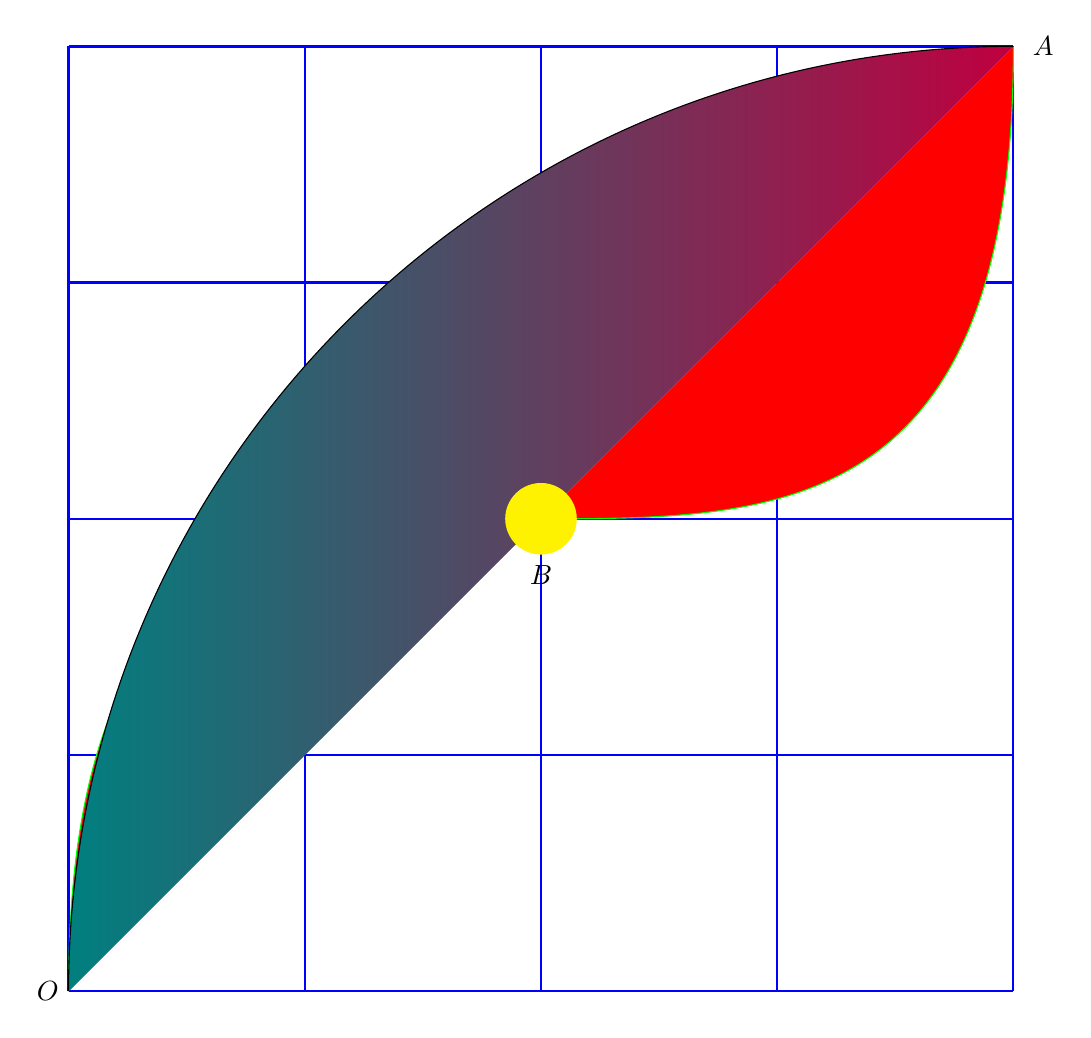
\begin{tikzpicture}[scale = 3]
	\draw[step = 1cm, blue, thick] (0,0) grid (4,4);
	\filldraw (0,0)[fill = red, draw = green] .. controls (0,4) and (4,0) .. (4,4);
	\shadedraw[left color = green!50!blue, right color = purple, draw = black] (0,0) arc (180:90:4cm);
	\node[anchor = east] at (0,0) {$O$};
	\node[label = 360:$A$] at (4,4) {};
	\node[circle, draw, fill, color = yellow, inner sep=3, label=270:$B$, scale=3] at (2,2) {};
\end{tikzpicture}

\section{Basic}
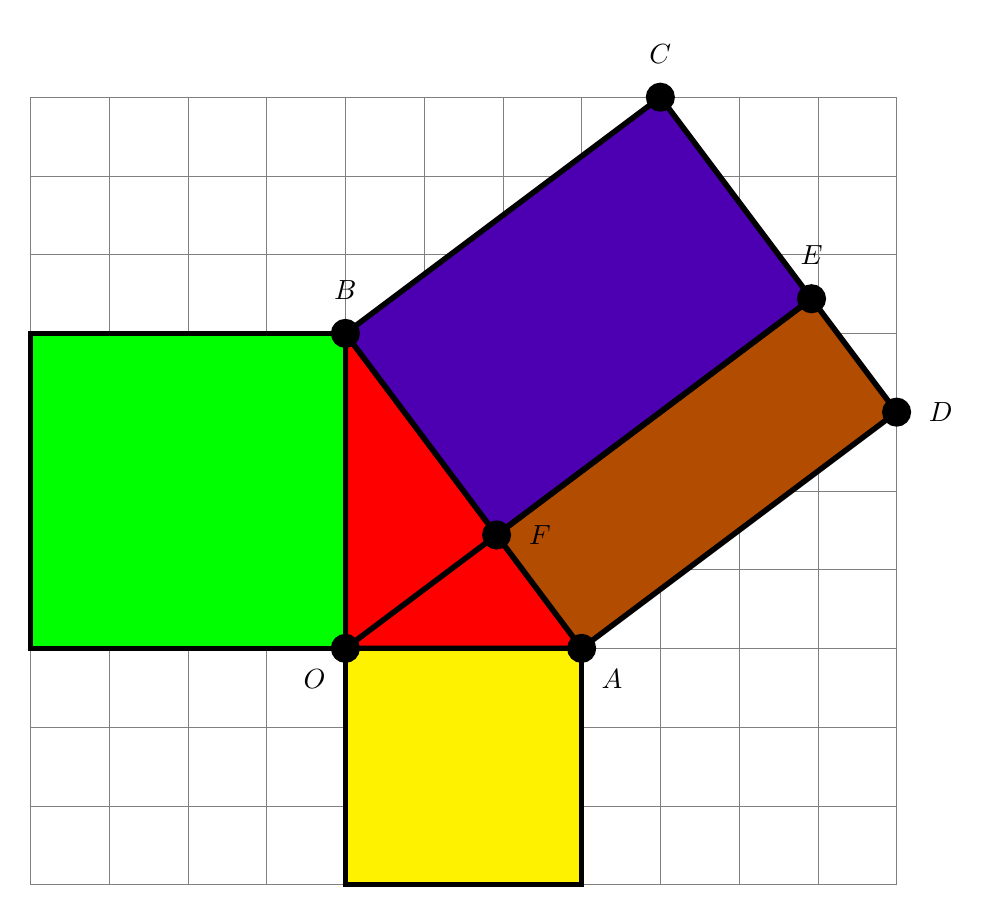
\begin{tikzpicture}[line width = 2pt]
	\newcommand{\la}{3}
	\newcommand{\lb}{4}
	\tikzstyle{every node} =[circle, draw, fill, inner sep=3]
	\draw[help lines] (-\lb,-\la) grid (\la+\lb,\la+\lb);
	\coordinate (O) at (0,0);
	\coordinate (A) at (\la,0);
	\coordinate (B) at (0,\lb);
	\coordinate (C) at ($(B) + (\lb,\la)$);
	\coordinate (D) at ($(A) + (\lb,\la)$);
	\coordinate (E) at ($(C)!(O)!(D)$);
	\coordinate (F) at ($(B)!(O)!(A)$);
	\draw[fill=red] (O) -- (A) -- (B) -- (O);
	\draw[fill=red!30!blue] (B) -- (C) -- (E) -- (F) -- (B);
	\draw[fill=green!30!red] (D) -- (E) -- (F) -- (A) -- (D);
	\draw[fill=yellow] (O) rectangle (\la,-\la);
	\draw[fill=green] (O) rectangle (-\lb,\lb);
	\draw (O) -- (E);
	\node[label=225:$O$] at (O) {};
	\foreach \v/\l in {A/315,B/90,C/90,D/360, E/90, F/0}
		{\node[label=\l:$\v$] at (\v) {}; }
\end{tikzpicture}

\section{Simple linear and parabolic function}
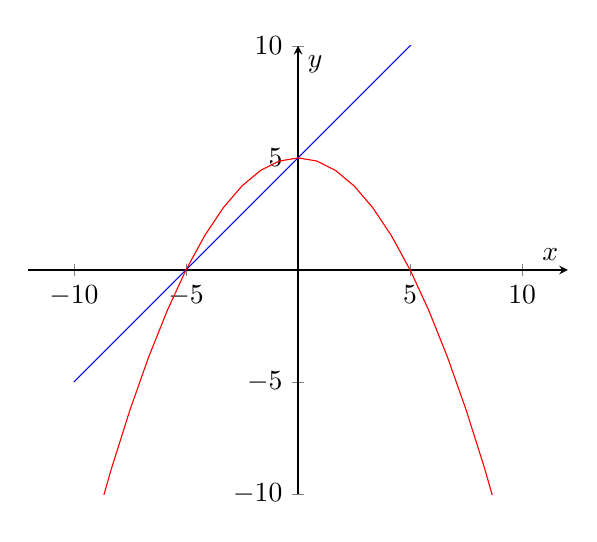
\begin{tikzpicture}
	\begin{axis}[xlabel=$x$,ylabel=$y$,xmin=-10, xmax=10, ymin=-10, ymax=10, axis lines=center, axis equal]
		\addplot[domain= -10:10, color=blue,] {x+5};
		\addplot[domain= -10:10, color=red, ] {-0.2*x^2+5};
	\end{axis}
\end{tikzpicture}

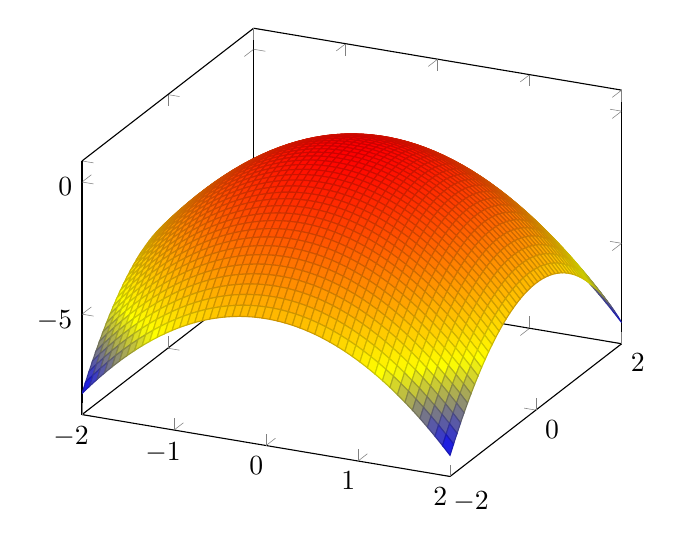
\begin{tikzpicture}
	\begin{axis}[samples=50]
		\addplot3[surf, domain=-2:2] {-x^2-y^2};
	\end{axis}
\end{tikzpicture}

\begin{tikzpicture}
	\draw[->] (-3,0) -- (4.2,0) node[right] {$x$};
	\draw[->] (0,-3) -- (0,4.2) node[above] {$y$};
	\draw[scale=0.5,domain=-3:3,smooth,variable=\x,blue] plot ({\x},{\x*\x});
	\draw[scale=0.5,domain=-3:3,smooth,variable=\y,red]  plot ({\y*\y},{\y});
\end{tikzpicture}

\end{document}